% 第5章 視線データセット
\newpage
\renewcommand{\baselinestretch}{1.5}
\section{視線データセット}
\renewcommand{\baselinestretch}{1}
\par ウェブページの左上から中央にかけての領域に注目が集まる現象として知られるf-biasのようなバイアスを考慮して正確な顕著性を予測するためにはユーザーがウェブページを閲覧する際の視線データセットが必要となる。ウェブ上に公開されている視線のデータセットはほとんど存在しておらず、近年のモダンデザインに対応しているものは存在しないためオリジナルデータセットを作成する。

\subsection{ウェブデータセット}\label{subsec:webdataset}
\par データセットに使用するウェブページについては昔のベーシックデザインだけでなくモダンなデザインも含まれており、日本語の様々なカテゴリーのウェブサイトのリンクをまとめているイケサイ\cite{ikesai}を使用して収集した。イケサイに掲載されている
「コーポレート」や「食」や「政治」などの幅広い27カテゴリからそれぞれランダムに10個ずつ取得した合計270個のウェブサイトのスクリーンショットをFirefoxブラウザのフルスクリーンモードの1280px×803pxで取得した。取得したウェブページデータセットの一部を図\ref{fig_webpage-dataset}に示す。

\begin{figure}[H]
  \centering
  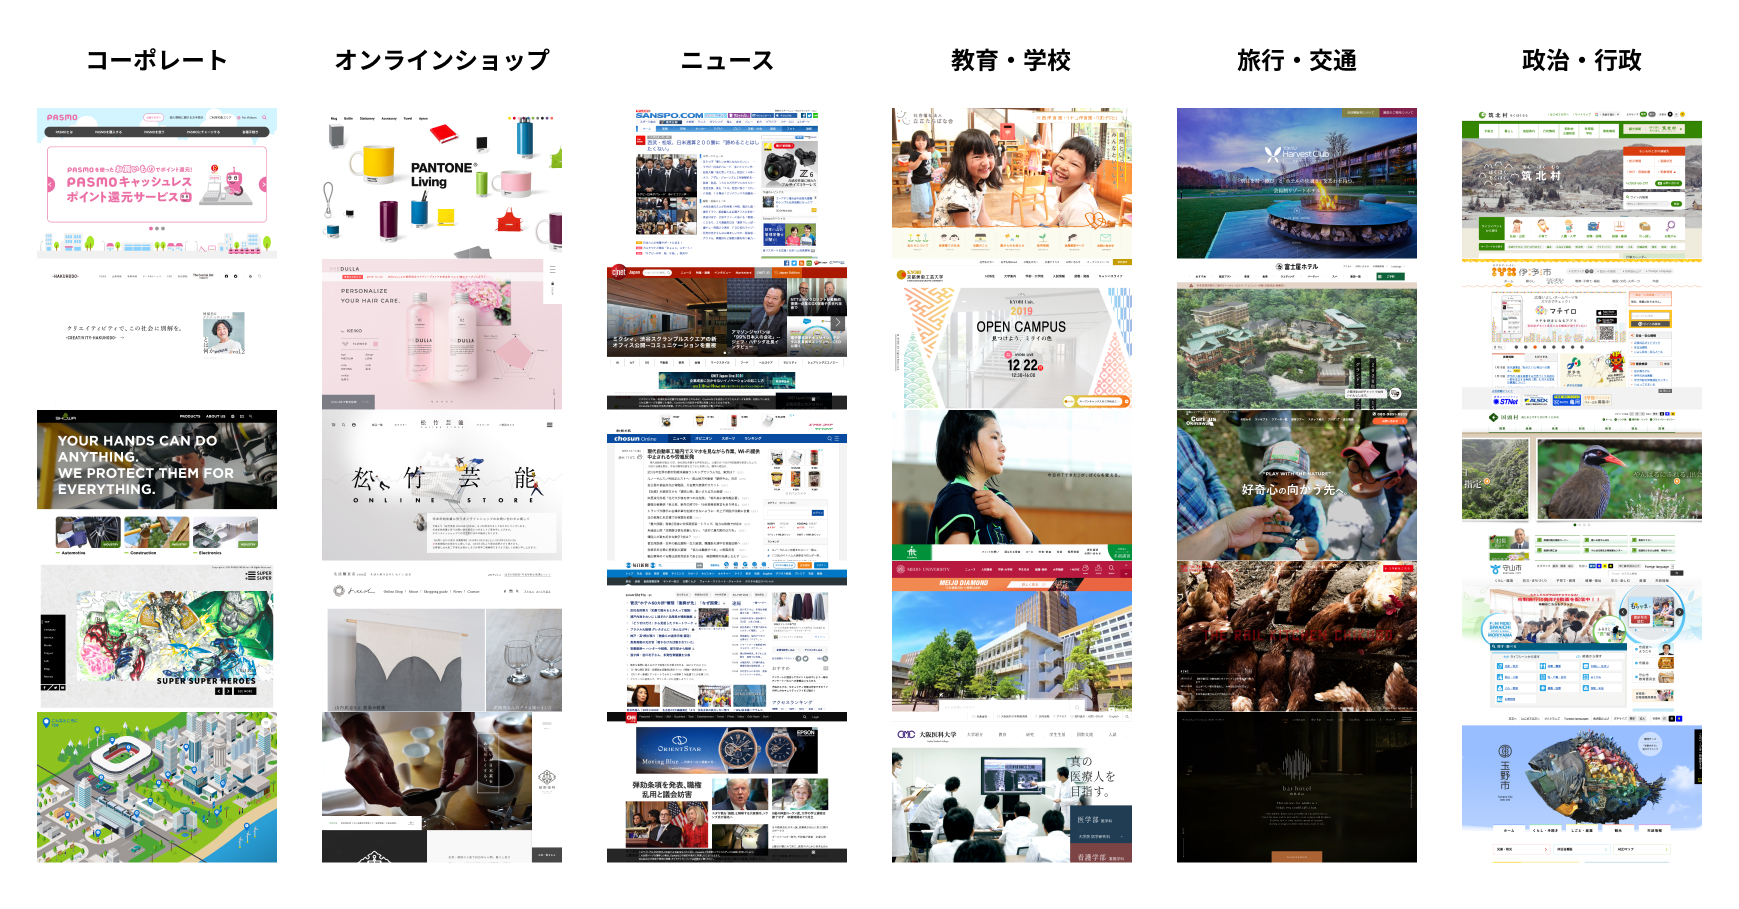
\includegraphics[width=12.5cm]{figures/05_dataset.jpg}
  \caption{データセットに含まれるウェブページの例}
  \label{fig_webpage-dataset}
\end{figure}

\par 収集したウェブサイトは日常で閲覧する多くのサイトをカバーできるように様々な異なるカテゴリから構成されており、被験者が実験中にレイアウトによる視線の偏りが発生することを防ぐことができる。


\subsection{アイトラッカーを使用した視線データ収集}\label{subsec:gazedataset}
\par 視線データ収集には19歳から26歳の合計35名(男性:27名、女性:8名)が参加した。被験者は日常でインターネットを使用するネットユーザーでいずれも健常者であった。

\par 視線データ収集はTobii Pro Nano\cite{tobiipronano}を使用して行い、被験者は1920px×1080pxの画面から60cm離れた位置でウェブページを閲覧した。ウェブページのスクリーンショットは画面の中央に最大サイズで表示して視線のデータはTobii Pro Lab\cite{tobiiprolabo}を使用して60Hzのサンプリングレートで記録された。各被験者は正確な視線データを記録するためにレコーディングを始める前にキャリブレーションを行った。その後ウェブデータセットの中からランダムにウェブページが10秒間表示され目的なしの自由状態で閲覧した。ウェブページを閲覧した後5秒間黒い画面が表示され、これらを合計20個のウェブページで実施した。各被験者はこれらのセットを休憩を挟んで合計2セット実施した。なお、各ウェブページは異なる5名の被験者によって閲覧された。


\subsection{データ分析}
\par 図\ref{fig_dataset-saliency}に収集したウェブページの凝視視線データの例をヒートマップで示す。各ウェブページのヒートマップは5名の被験者のウェブページの視線データをTobii Pro Labで半径50pxのTobii I-VT Gaze Filterを用いて作成した。ウェブページのレイアウトによって視線が集まる領域は様々で、特に左上から中央付近にかけて視線が集まりやすいことが分かる。また、人物が映る写真が存在する場合、顔付近に注目が集まりやすい傾向があることも分かる。

\par これらの視線座標の傾向を分析するために私たちは特に視線座標との関係性が高いウェブページ固有のレイアウトに着目して第\ref{subsec:webdataset}節で作成したウェブデータセットをレイアウトパターンに分類した。既存研究でウェブページのレイアウトパターンを定義しているものが存在しないため、Webデザイン、これからどうなるの?\cite{bookwebdesign}などの書籍やウェブページレイアウトについてまとめられたサイトから視線のパターンを考慮して既存のウェブページレイアウトをカバーできるように表\ref{table:layoutpattern}に示す合計7パターンに決定した。また、それぞれのレイアウトパターンに該当するウェブページの例を図\ref{fig_layout_example}に示す。オーソドックスなブログのようなシングルカラムのデザインやニュースメディアなどの複数のカラムを持つカラムデザイン、さらに全画面の画像にテキストなどの要素を散りばめたモダンデザインまでウェブページのレイアウトで分類を行う事が可能である。

\begin{figure}[H]
  \centering
  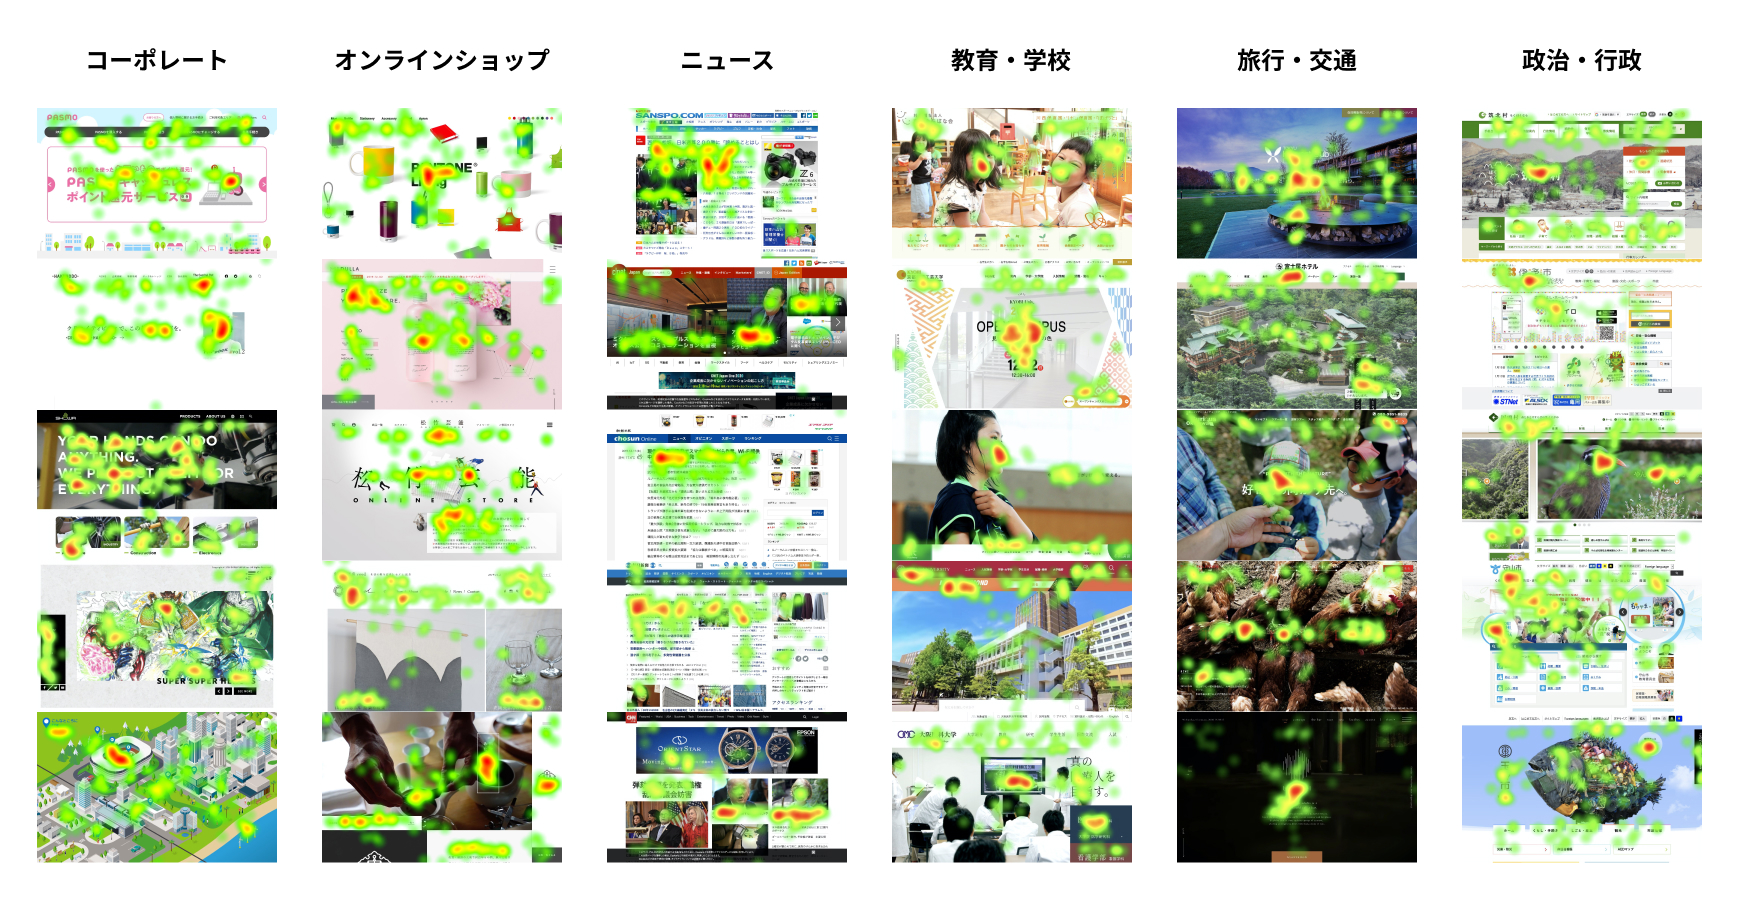
\includegraphics[width=12.5cm]{figures/05_dataset_saliency.jpg}
  \caption{記録した視線データの例}
  \label{fig_dataset-saliency}
\end{figure}

\begin{table}[h]
  \caption{ウェブページレイアウトパターンの一覧}
  \label{table:layoutpattern}
  \centering
    \begin{tabular}{clll}
    \hline
    パターン名 & 説明 \\
    \hline \hline
    シングルカラム & ページが一列で構成されるレイアウト \\
    2カラム & ページが二列で構成されるレイアウト \\
    3カラム & ページが三列で構成されるレイアウト \\
    4カラム & ページが四列で構成されるレイアウト \\
    カードレイアウト & カードのようなブロック要素が並べられるレイアウト \\
    ブロークングリッド & 要素が画面の様々な位置に散りばめられたモダンデザイン \\
    フルスクリーン & 画面全体にトップビューが広がるモダンデザイン \\
    \hline
  \end{tabular}
\end{table}

\begin{figure}[H]
  \centering
  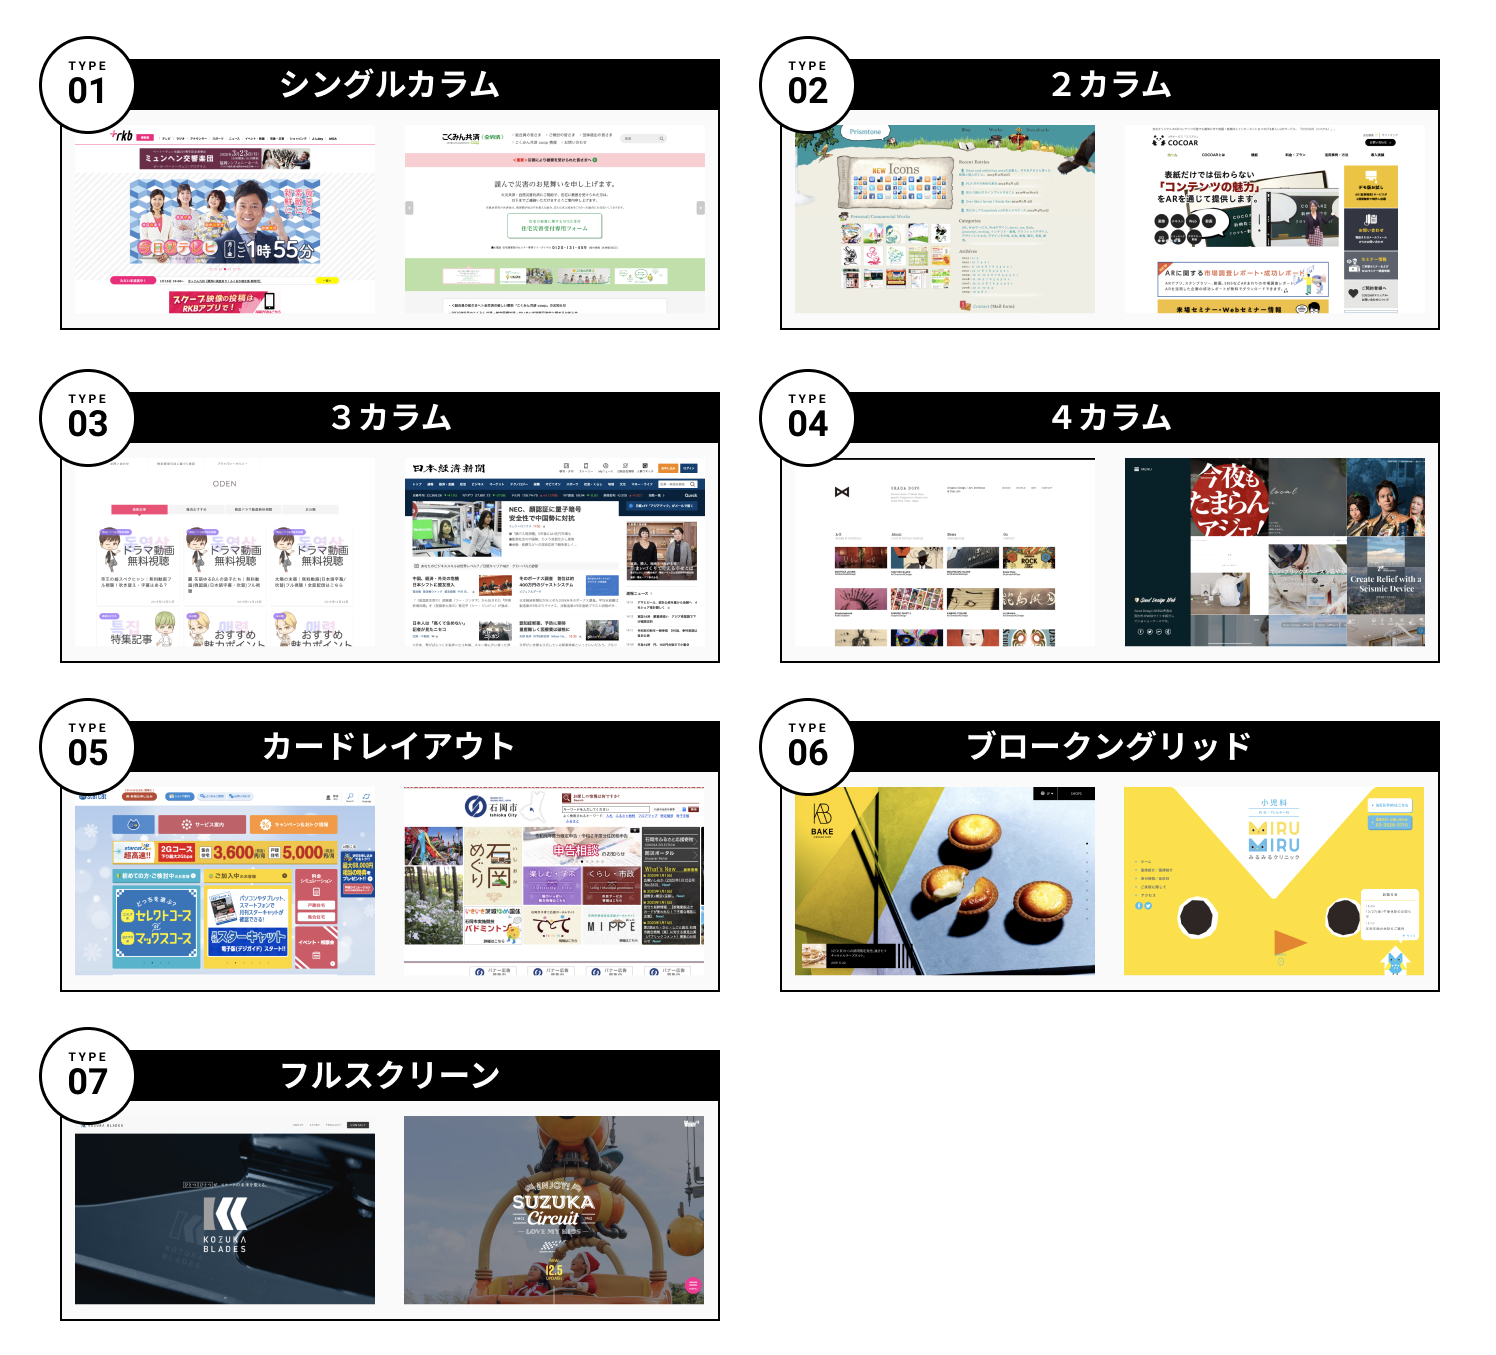
\includegraphics[width=10cm]{figures/05_layout.jpg}
  \caption{各レイアウトパターンに該当するウェブページの例}
  \label{fig_layout_example}
\end{figure}

\par 私たちは第\ref{subsec:gazedataset}節で収集した270個のウェブページの視線データセットをランダムに4:1に分類して216個のウェブページの視線データセットをデータ分析用に使用し、残りの54個を評価実験用に使用した。ここではデータ分析用の216個のウェブページを先ほど説明した7個のレイアウトパターンに分類して分析を行う。

\par 被験者は各ウェブページを10秒間閲覧したが、視線座標の推移の分析により閲覧時間によって大きく視線が移動する事が判明した。そこで、各レイアウトパターンごとの視線データの動きの傾向を分析するために被験者の10秒間の視線データを2秒ごとに0-2秒, 2-4秒, 4-6秒, 6-8秒, 8-10秒の5つに分割してそれぞれの時間帯での注視点の座標の位置を分析する。まず初めに各ウェブページ毎に各時間帯ごとの視線座標の平均を計算してこれを平均座標と呼ぶ。さらに各レイアウトパターン毎に該当するウェブページ全ての平均座標の平均を計算したものを中央点と呼ぶ。中央点は各レイアウトパターンのウェブページの時間帯毎の平均の視線座標の位置を示しており、これにより視線座標の推移を認識する事が可能である。また、各時間帯毎の全てのウェブページの平均座標が含まれる円を計算した。表\ref{table:layoutresult}に各パターンの時間帯ごとの注視点の平均座標である中央点と座標が含まれる円の半径を示す。さらに図\ref{fig_layout_result}に各ウェブページの中央点と各レイアウトごとの中央点の移動の軌跡を示す。ピンク色の円は各時間帯毎の楕円を示しており、赤色の線は中央点の移動の軌跡を示している。

\begin{table}[h]
  \caption{各パターンの時間帯ごとの中心点座標とその半径}
  \label{table:layoutresult}
  \footnotesize
  \centering
    \begin{tabular}{clllll}
    \hline
    パターン名 & 秒数 & 中央点X[px] & 中央点Y[px] & 半径X[px] & 半径Y[px] \\
    \hline \hline
    \multirow{5}{*}{シングルカラム} & 0-2s & 556.53526 & 368.23793 & 444.82839 & 237.78349 \\
    & 2-4s & 680.65559 & 438.25877 & 466.89552 & 308.36171 \\
    & 4-6s & 707.52981 & 496.78213 & 349.64802 & 278.91648 \\
    & 6-8s & 768.12999 & 511.91153 & 408.86725 & 338.98615 \\
    & 8-10s & 788.44816 & 515.60635 & 389.02887 & 352.11794 \\
    \hline
    \multirow{5}{*}{2カラム} & 0-2s & 537.90889 & 327.89538 & 371.11744 & 84.03475 \\
    & 2-4s & 638.07192 & 436.23222 & 396.09261 & 131.80240 \\
    & 4-6s & 673.81014 & 500.41143 & 382.18434 & 202.55096 \\
    & 6-8s & 748.26660 & 563.43498 & 338.23595 & 204.41473 \\
    & 8-10s & 738.18496 & 583.13415 & 359.40345 & 226.29391 \\
    \hline
    \multirow{5}{*}{3カラム} & 0-2s & 553.66790 & 375.01389 & 156.00054 & 74.33003 \\
    & 2-4s & 630.30464 & 442.51196 & 197.01774 & 190.90868 \\
    & 4-6s & 740.487670 & 524.98878 & 250.85640 & 172.198448 \\
    & 6-8s & 692.25816 & 558.33862 & 371.49920 & 154.66621 \\
    & 8-10s & 729.13148 & 544.05520 & 271.23804 & 152.74239 \\
    \hline
    \multirow{5}{*}{4カラム} & 0-2s & 622.93684 & 403.41291 & 39.81908 & 23.29113 \\
    & 2-4s & 652.95710 & 587.20462 & 57.61500 & 43.52946 \\
    & 4-6s & 550.20828 & 680.73009 & 119.84877 & 132.47447 \\
    & 6-8s & 741.04658 & 624.54582 & 129.73321 & 175.20079 \\
    & 8-10s & 926.99540 & 530.66825 & 172.67673 & 87.60673 \\
    \hline
    \multirow{5}{*}{カードレイアウト} & 0-2s & 569.89335 & 310.07291 & 248.88284 & 51.79706 \\
    & 2-4s & 612.14546 & 391.96698 & 399.64150 & 78.47047 \\
    & 4-6s & 688.60131 & 481.16412 & 166.22500 & 119.72984 \\
    & 6-8s & 723.86810 & 507.66301 & 216.52019 & 128.41249 \\
    & 8-10s & 782.71513 & 540.81882 & 194.26017 & 152.85102 \\
    \hline
    \multirow{5}{*}{ブロークングリッド} & 0-2s & 645.74007 & 458.44231 & 466.02712 & 326.28638 \\
    & 2-4s & 682.06057 & 494.16684 & 596.61873 & 335.88933 \\
    & 4-6s & 740.43617 & 500.64521 & 522.82219 & 322.04717 \\
    & 6-8s & 783.37446 & 520.62385 & 530.18073 & 292.10090 \\
    & 8-10s & 759.12313 & 529.81126 & 360.04529 & 305.44824 \\
    \hline
    \multirow{5}{*}{フルスクリーン} & 0-2s & 640.26711 & 423.96134 & 298.25324 & 184.01572 \\
    & 2-4s & 673.68514 & 472.42480 & 359.91272 & 197.11066 \\
    & 4-6s & 672.59751 & 542.48711 & 497.06624 & 264.81229 \\
    & 6-8s & 694.48142 & 545.09160 & 389.88440 & 221.83996 \\
    & 8-10s & 722.54375 & 520.62472 & 484.22990 & 333.35191 \\
    \hline
  \end{tabular}
\end{table}

\begin{figure}[H]
  \centering
  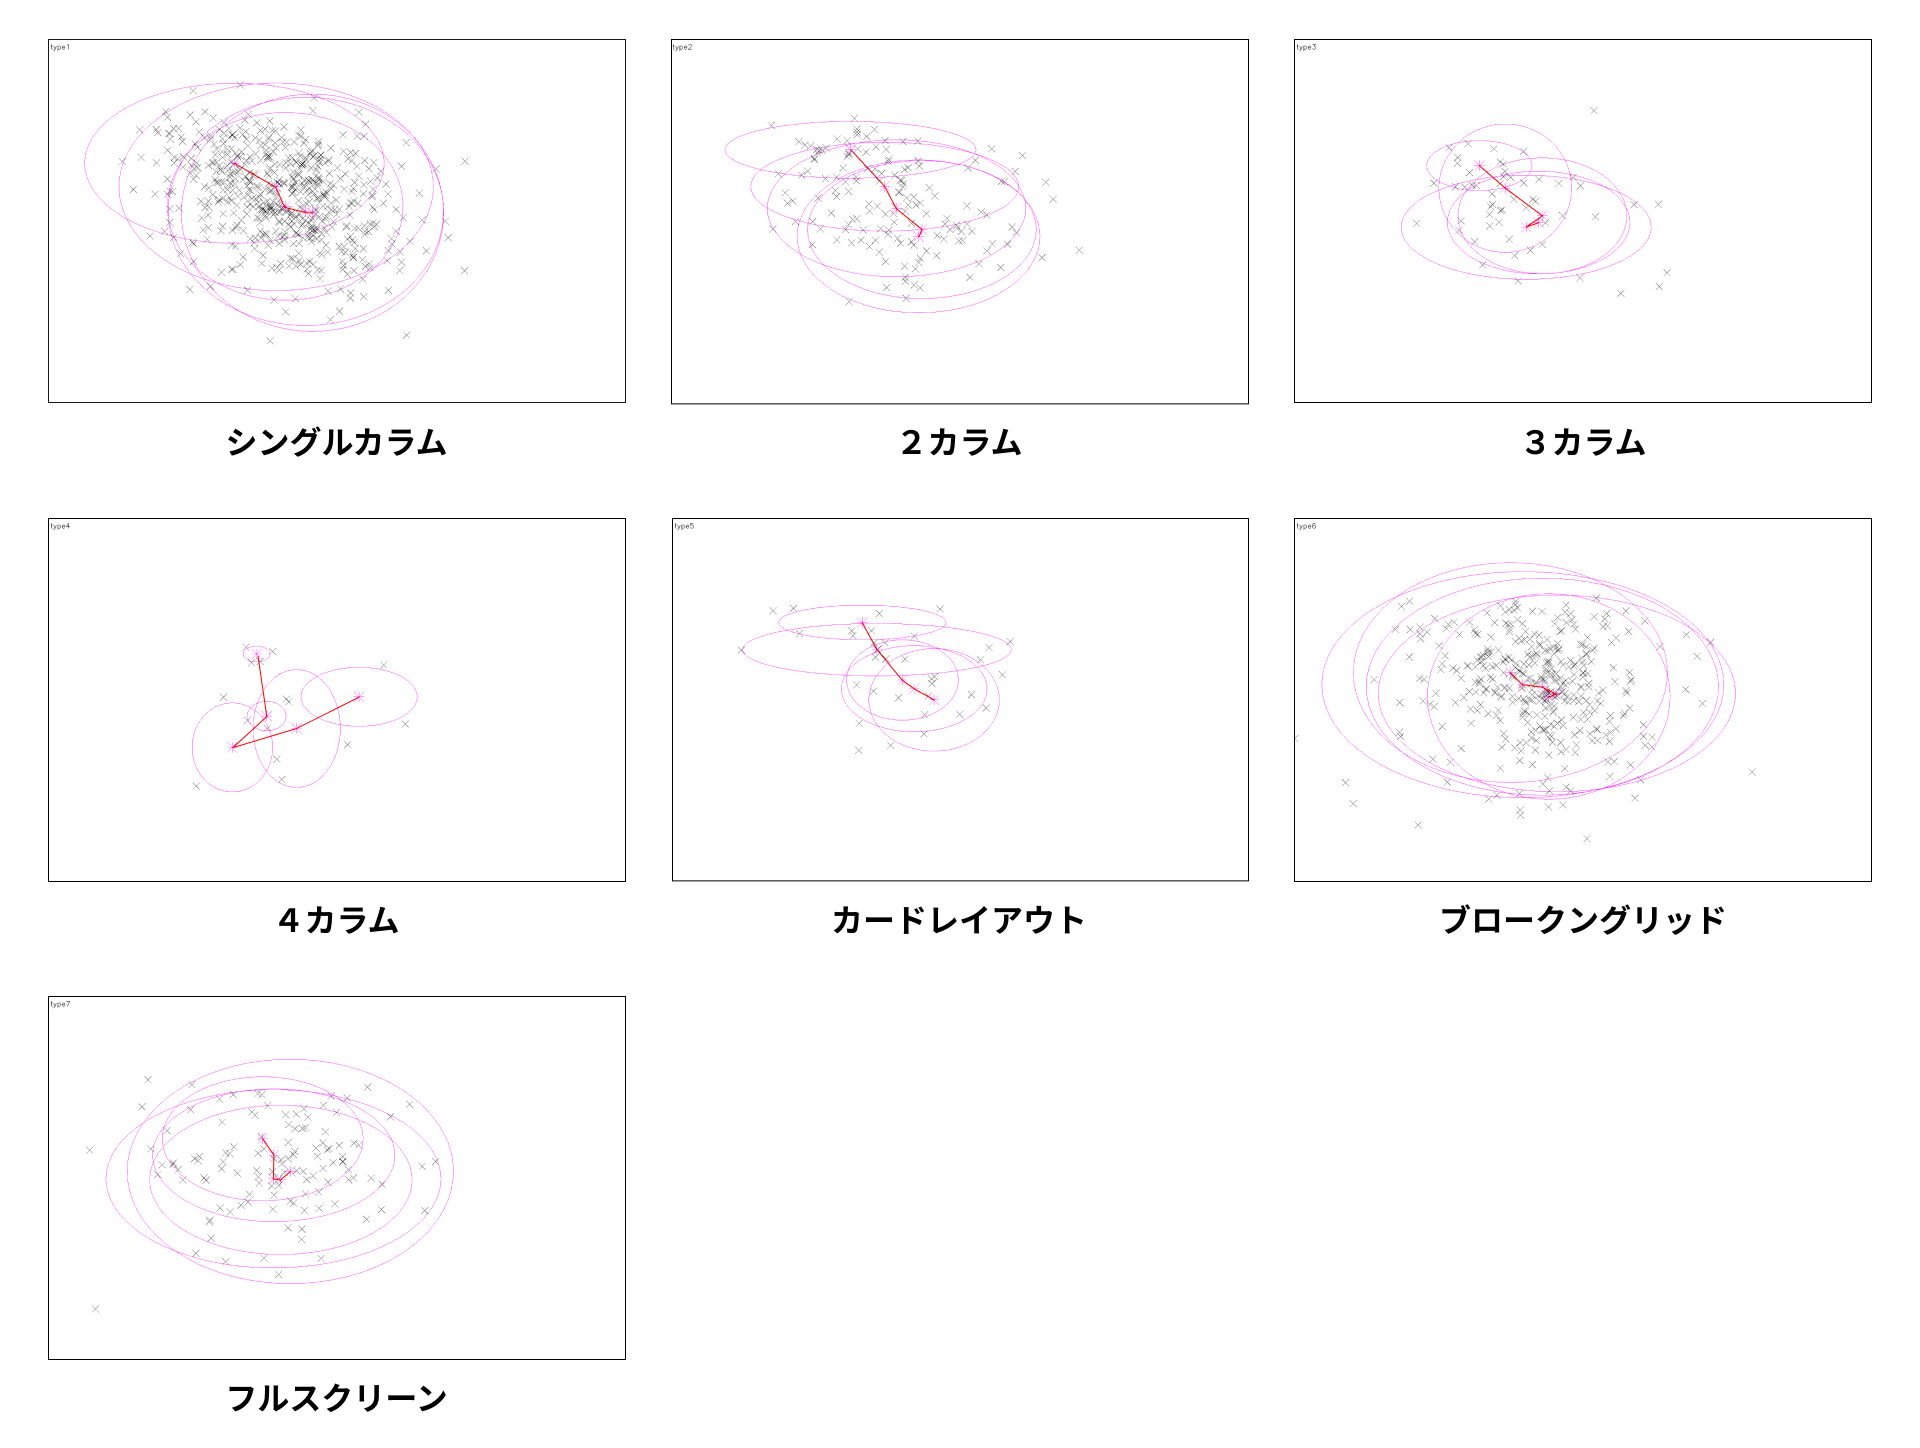
\includegraphics[width=12cm]{figures/05_layout_result.jpg}
  \caption{ウェブページのレイアウト分類結果}
  \label{fig_layout_result}
\end{figure}

\par 図\ref{fig_layout_result}を見ると各レイアウトパターン毎に。。。

ToDo: 各パターン毎の特徴を記述、全体でわかったことも記述
ToDo: 中央点の計算方法に関しては数式で記述した方が良いかも
